\documentclass[a4paper,11pt]{article}

% Codificación e idioma
\usepackage[utf8]{inputenc}
\usepackage[T1]{fontenc}
\usepackage[spanish,es-tabla,es-noshorthands]{babel}
% Hace que \% sea el signo de porcentaje plano (evita el error de
% babel-spanish "Incompatible glue units" cuando aparece en modo mat.)
\spanishplainpercent

% Geometría
\usepackage[a4paper,margin=2.5cm]{geometry}

% Matemáticas
\usepackage{amsmath,amssymb,mathtools}

% Gráficos y tablas
\usepackage{graphicx}
\graphicspath{{assets/}{./}}
\usepackage{booktabs}
\usepackage{array}
\usepackage{float}

% Tipografía y listas
\usepackage{lmodern}
\usepackage{microtype}
\usepackage{enumitem}
\setlist[itemize]{leftmargin=*,itemsep=2pt,topsep=2pt}
\setlist[enumerate]{leftmargin=*,itemsep=2pt,topsep=2pt}

% Color
\usepackage{xcolor}

% Bibliografía
\usepackage{natbib}
\bibliographystyle{plainnat}

% Enlaces (cargar al final)
\usepackage{hyperref}
\hypersetup{colorlinks=true,linkcolor=black,urlcolor=blue!75!black,citecolor=blue!75!black,
            pdftitle={Informe: Enhanced Prediction of Electricity Peak Load},
            pdfauthor={Grupo de trabajo}}

% Espaciado de párrafos (sin sangría francesa)
\setlength{\parindent}{0pt}
\setlength{\parskip}{0.55em}

% Cajas de nota y aviso
\newcommand{\notebox}[1]{\par\medskip\noindent%
  \colorbox{blue!8}{\parbox{\dimexpr\linewidth-2\fboxsep\relax}{\textbf{Nota.} #1}}%
  \par\medskip}
\newcommand{\warnbox}[1]{\par\medskip\noindent%
  \colorbox{orange!18}{\parbox{\dimexpr\linewidth-2\fboxsep\relax}{#1}}%
  \par\medskip}

\begin{document}

% =====================================================================
% PRIMERA PÁGINA: título, autores, resumen, problema, objetivos,
% preguntas y justificación.
% =====================================================================

\begin{center}
	{\Large\bfseries Enhanced Prediction of Electricity Peak Load\\[0.2em]
		via Machine Learning and Time Series Analysis\par}
	\vspace{0.35em}
	{\small Grupo 3 \quad\textbullet\quad 2 de julio de 2026\par}
\end{center}
\vspace{0.5em}

\section*{Datos del artículo}

\noindent\textbf{Autores:} S.~Suriya \& R.~Agusthiyar\\
\textbf{Afiliación:} Department of Computer Science and Applications, SRM Institute of Science and Technology, Ramapuram Campus, Chennai, India.\\
\textbf{Publicación:} ZANCO Journal of Pure and Applied Sciences (2026), 38(2): 197 a 211.\\
\textbf{DOI:} \href{https://doi.org/10.21271/ZJPAS.38.2.14}{10.21271/ZJPAS.38.2.14}\\
\textbf{Palabras clave:} ARIMA, Multivariate, Lasso, XGR Regressor.

\section*{Resumen}

El artículo aborda el pronóstico de la demanda máxima (pico) de electricidad en Tamil Nadu, India, problema crítico para la estabilidad de la red, la programación de la generación y la planificación energética. La dificultad proviene de la estacionalidad, el crecimiento económico y las anomalías climáticas de la región. La metodología propone un marco híbrido que integra modelos estadísticos de series temporales (ARIMA y VAR) con modelos de aprendizaje automático (Lasso, Ridge y XGBoost), aplicados a datos mensuales de consumo y variables meteorológicas. El preprocesamiento incluyó imputación, detección de atípicos (Winsorización), normalización Min-Max y codificación cíclica; la ingeniería de variables incorporó rezagos, medias móviles, razones sectoriales y términos de interacción. Los modelos se evaluaron con MAE, RMSE y MAPE mediante validación walk-forward y $k$-fold. Los resultados muestran que el modelo híbrido propuesto alcanzó el menor error (MAPE $3{,}82\,\%$), seguido por ARIMA ($6{,}28\,\%$) y VAR ($7{,}82\,\%$), aunque el resumen del artículo atribuye el mejor desempeño a ARIMA.

\section*{Planteamiento del problema}

La predicción del pico de demanda eléctrica es esencial para garantizar un suministro confiable, optimizar la operación de la red y prevenir apagones. En Tamil Nadu, la demanda presenta patrones complejos por la combinación de estacionalidad (calor extremo, monzones), crecimiento económico y prácticas socio-culturales. Los modelos estadísticos tradicionales (ARIMA simple, suavizado exponencial) capturan tendencia y estacionalidad lineales pero fallan en interacciones multivariable complejas; los modelos de aprendizaje automático son flexibles pero propensos al sobreajuste, poco interpretables y exigentes en datos. Los enfoques híbridos existentes carecen de optimización sistemática y no superan de forma consistente a modelos únicos bien calibrados.

\section*{Objetivos}

\noindent\textbf{Objetivo general.} Desarrollar un marco de pronóstico híbrido que integre modelos estadísticos de series temporales y de aprendizaje automático para predecir la demanda máxima mensual de electricidad en Tamil Nadu.

\noindent\textbf{Objetivos específicos:}
\begin{enumerate}
	\item Integrar ARIMA, VAR y un ensemble híbrido VAR-ML (Lasso, Ridge, XGBoost) para capturar dependencias lineales y no lineales.
	\item Aplicar el marco a datos históricos de consumo eléctrico y variables meteorológicas de Tamil Nadu.
	\item Evaluar comparativamente los modelos con RMSE, MAE, MAPE y el estadístico $U$ de Theil.
	\item Demostrar la utilidad del modelo para planificación operativa, gestión de carga y formulación de política.
\end{enumerate}

\section*{Preguntas de investigación}

\begin{enumerate}
	\item ¿En qué medida un marco híbrido supera a los modelos individuales (ARIMA, VAR, Lasso, Ridge, XGBoost) en la predicción del pico de demanda mensual?
	\item ¿Qué variables (meteorológicas, sectoriales) contribuyen más a la precisión del pronóstico?
	\item ¿Cómo se comporta el modelo durante meses con anomalías climáticas extremas?
	\item ¿Es el modelo utilizable por operadores de red para decisiones operativas y de política?
\end{enumerate}

\section*{Justificación}

La predicción precisa del pico de demanda permite a las empresas eléctricas programar la generación, equilibrar la carga, realizar mantenimiento preventivo en períodos de baja demanda y dimensionar la infraestructura de almacenamiento y generación. Para Tamil Nadu, donde el clima y la dinámica industrial afectan el consumo, un modelo calibrado localmente aporta valor operativo y de política. Además, el estudio integra factores socio-económicos y climáticos poco considerados en la literatura regional, y busca un balance entre interpretabilidad y precisión, condición clave para la adopción por parte de los decisores del sector eléctrico.

\newpage
\section*{Metodología estadística}

\subsection*{Descripción del conjunto de datos}

El conjunto se obtuvo del portal de datos abiertos de la empresa eléctrica estatal de Tamil Nadu. Comprende registros mensuales de enero de 2018 a diciembre de 2022 e incluye: fecha; consumo total (MWh); consumo sectorial (residencial, industrial, agrícola, comercial); demanda máxima (MW); energía suministrada (MWh); número de consumidores por sector; y variables meteorológicas (temperatura media, humedad y precipitación) del Tamil Nadu State Climate Portal.

\notebox{El resumen del artículo indica datos de abril de 2006 a marzo de 2023, mientras que la sección 3.1 los restringe a 2018 a 2022. Esta inconsistencia se retoma en el análisis de resultados.}

\subsection*{Preprocesamiento de datos}

\begin{itemize}
  \item \textbf{Imputación de valores faltantes:} combinación de interpolación lineal (para brechas cortas) y \textit{forward-fill} (para brechas largas).
  \item \textbf{Detección de atípicos:} $Z$-score (umbral $|z|>3$) y rango intercuartílico (IQR); los valores extremos se \textit{winsorizaron} en los percentiles 5 y 95.
  \item \textbf{Normalización:} Min-Max al rango $[0,1]$ para equiparar escalas.
  \item \textbf{Codificación temporal cíclica:} seno y coseno para mes y año, preservando la periodicidad:
\end{itemize}
\[ \text{month}_{\sin}=\sin\!\left(\frac{2\pi\cdot\text{month}}{12}\right),\qquad
   \text{month}_{\cos}=\cos\!\left(\frac{2\pi\cdot\text{month}}{12}\right) \]

\subsection*{Ingeniería de variables}

\begin{itemize}
  \item \textbf{Rezagos (\textit{lags}):} 1, 3 y 6 meses del consumo y de la demanda máxima.
  \item \textbf{Medias móviles (\textit{rolling}):} medias de 3 y 6 meses.
  \item \textbf{Razones sectoriales:} residencial/industrial y comercial/total.
  \item \textbf{Términos de interacción:} Temperatura $\times$ Humedad y Desviación de precipitación $\times$ Energía suministrada.
  \item \textbf{Métricas de cambio porcentual:} variación mensual del consumo y de la demanda.
\end{itemize}

\subsection*{Modelos estadísticos y de aprendizaje automático}

\noindent\textbf{Modelos basados en variables (regresión).}

\textit{Lasso} (regularización L1):
\[ \hat{\beta}=\arg\min_{\beta}\left\{\sum_{i=1}^{n}(y_i-X_i\beta)^2+\lambda\|\beta\|_1\right\} \]

\textit{Ridge} (regularización L2):
\[ \hat{\beta}=\arg\min_{\beta}\left\{\sum_{i=1}^{n}(y_i-X_i\beta)^2+\lambda\|\beta\|_2^2\right\} \]

\textit{XGBoost} (\textit{ensemble tree boosting}):
\[ \hat{y}_i=\sum_{k=1}^{K} f_k(x_i),\qquad \Omega(f)=\gamma T+\frac{1}{2}\lambda\|w\|^2 \]

\noindent\textbf{Modelos temporales.}

\textit{ARIMA$(p,d,q)$:}
\[ \phi(B)(1-B)^d\, y_t=\theta(B)\,\varepsilon_t \]
con $\phi(B)=1-\phi_1 B-\cdots-\phi_p B^p$ y $\theta(B)=1+\theta_1 B+\cdots+\theta_q B^q$, donde $B$ es el operador de retroceso.

\textit{VAR$(p)$} (para entrada multivariable):
\[ Y_t=c+\sum_{i=1}^{p} A_i\, Y_{t-i}+\varepsilon_t,\qquad Y_t\in\mathbb{R}^k,\; A_i\in\mathbb{R}^{k\times k},\; \varepsilon_t\sim\mathcal{N}(0,\Sigma) \]

\subsection*{Algoritmo híbrido propuesto}

El marco combina un componente de aprendizaje automático $M_{ML}\in\{\text{Lasso, Ridge, XGBoost}\}$ y uno de series temporales $M_{TS}\in\{\text{ARIMA, VAR}\}$. Sobre la matriz de variables enriquecida $X'$ se obtiene $\hat{y}_{ML}$; sobre la serie $y_t$ se obtiene $\hat{y}_{TS}$. La predicción final se selecciona minimizando una métrica de error $\varepsilon$ (RMSE o MAE) \citep{zhang2003}:
\[ \hat{y}_{final}=\arg\min_{\hat{y}\in\{\hat{y}_{ML},\,\hat{y}_{TS}\}}\varepsilon(y,\hat{y}) \]

\subsection*{Validación y selección de modelos}

\begin{itemize}
  \item Partición 80/20: entrenamiento 2018 a 2021, prueba 2022.
  \item \textbf{Walk-forward} (\textit{rolling-origin}) para ARIMA y VAR, preservando la integridad temporal.
  \item \textbf{Grid search + $k$-fold} ($k=5$) para Lasso, Ridge y XGBoost; el parámetro $\lambda$ se optimizó en escala logarítmica.
  \item \textbf{Estacionariedad:} test ADF (se diferenció si $p>0.05$).
  \item \textbf{Selección de rezagos:} AIC, BIC y HQIC, apoyada en ACF y PACF.
  \item \textbf{Diagnóstico de residuos:} test de Ljung-Box.
  \item \textbf{Métricas de desempeño:} MAE, RMSE, MAPE e intervalos de confianza al 95\,\%.
\end{itemize}

\newpage
\section*{Análisis de los resultados}

\subsection*{Resultados reportados}

La sigueinte tabla reune los resultados de las metricas de RMSE, MAE Y MAPE de todos los modelos individuales y los compara con el modelo hibrido:

\begin{table}[H]
\centering
\caption{Comparación entre el modelo propuesto, modelos base y estudios previos (tabla 4 del artículo).}
\label{tab:full}
\begin{tabular}{lccc}
\toprule
Modelo / Estudio & RMSE & MAE & MAPE (\%) \\
\midrule
Híbrido propuesto  & 112{,}35 & 85{,}27  & 3{,}82 \\
XGBoost            & 125{,}87 & 95{,}14  & 4{,}35 \\
Pandoh et al. (2021) & 128{,}67 & 97{,}53  & 4{,}40 \\
ARIMA              & 138{,}46 & 102{,}28 & 4{,}92 \\
VAR                & 140{,}82 & 104{,}37 & 5{,}03 \\
Ridge              & 142{,}33 & 107{,}84 & 5{,}09 \\
Lasso              & 145{,}62 & 110{,}45 & 5{,}21 \\
Kong et al. (2019) & 152{,}13 & 115{,}64 & 5{,}85 \\
\bottomrule
\end{tabular}
\end{table}
El modelo hibrido supera a todos los demas modelos en todas las métricas: menor MAE (85{,}27), menor RMSE (112{,}35) y menor MAPE ($3{,}82\,\%$ ),La figura~\ref{fig:peak} muestra la evolución del pico de demanda a lo largo del período estudiado.

\begin{figure}[H]
\centering
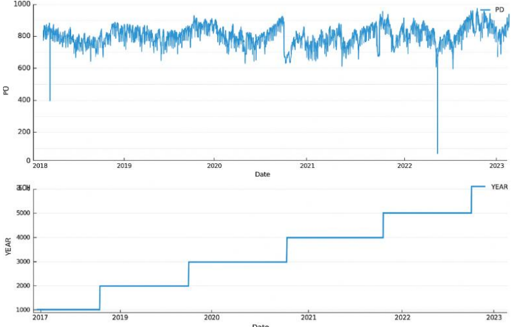
\includegraphics[width=0.5\linewidth]{fig1_peak_demand.png}
\caption{Demanda máxima de electricidad por año (figura 1 del artículo original).}
\label{fig:peak}
\end{figure}
 Los resultados obtenidos son consistentes con las conclusiones del artículo de referencia, ya que el modelo híbrido volvió a ser la alternativa con mayor precisión frente a los modelos individuales. Aunque el orden de desempeño de ARIMA, VAR, Lasso y XGBoost difiere del reportado por Suriya y Agusthiyar (2026), debido a que el presente estudio utiliza un conjunto de datos distinto (Países Bajos en lugar de Tamil Nadu), se confirma que la integración de modelos estadísticos y de aprendizaje automático permite reducir el error de pronóstico. Esto evidencia que el enfoque híbrido posee una mayor capacidad para adaptarse a diferentes patrones de consumo eléctrico, constituyéndose como la estrategia más robusta para la predicción de la demanda máxima.

\newpage
% =====================================================================
% QUINTA Y SEXTA PÁGINA: aplicación de la metodología con datos y análisis
% de los resultados correspondientes.
% =====================================================================

\section*{Aplicación de la metodología}

\subsection*{Datos}

Se aplicó la metodología del artículo a un conjunto de datos sintético de consumo y clima (datos diarios de 20 países, 2020 a 2024). Siguiendo los lineamientos del artículo, se trabajó en frecuencia mensual y se eligió el país más pequeño del conjunto: Países Bajos. El proceso de limpieza deja un conjunto depurado mediante los siguientes pasos:

\begin{itemize}
  \item Filtrado por país, con la fecha como índice temporal, verificación de continuidad diaria y de valores faltantes (no había).
  \item Agregación mensual: la variable objetivo es el pico de consumo mensual, es decir, el máximo diario de consumo en cada mes (análogo al pico de demanda del artículo); como exógenas se usan la temperatura y la humedad medias del mes.
  \item Winsorización mensual (percentiles 5 y 95) sobre las series agregadas, de modo que solo se recorten los meses extremos.
\end{itemize}

\noindent El resultado son 60 observaciones mensuales, de enero de 2020 a diciembre de 2024.

\subsection*{Metodología aplicada}

Se replicaron los pasos del artículo: test ADF de estacionariedad (diferenciando si $p>0{,}05$), selección de órdenes por AIC, validación walk-forward sobre 2024 (horizonte $h=1$, reestimando en cada paso) y métricas MAE, RMSE y MAPE.

\begin{itemize}
  \item ARIMA: los órdenes $(p,d,q)$ se seleccionaron automáticamente minimizando el AIC, con estacionalidad anual. El modelo elegido fue ARIMA$(0,1,1)(1,1,0)_{12}$, con AIC $510{,}7$. El test de Ljung-Box sobre los residuos arrojó $p=0{,}0007$, por lo que aún queda autocorrelación residual por capturar.
  \item VAR: modelo multivariado sobre el pico de consumo, la temperatura y la humedad (diferenciadas para garantizar estacionariedad conjunta). El rezago se eligió por AIC y resultó ser 6 (AIC $12{,}6$). El Ljung-Box sobre los residuos del pico dio $p=0{,}62$, es decir, sin autocorrelación residual.
\end{itemize}

\subsection*{Resultados}

\begin{table}[H]
\centering
\caption{Desempeño comparativo de ARIMA y VAR sobre el pico mensual (Países Bajos, validación walk-forward 2024).}
\label{tab:app}
\begin{tabular}{lccccc}
\toprule
Modelo & Órdenes / rezago & AIC & MAE & RMSE & MAPE (\%) \\
\midrule
ARIMA & $(0,1,1)(1,1,0)_{12}$ & 510{,}7 & 324{,}71 & 373{,}99 & 2{,}64 \\
VAR   & rezago 6 & 12{,}6 & 345{,}09 & 463{,}83 & 3{,}26 \\
\bottomrule
\end{tabular}
\end{table}

\begin{figure}[H]
\centering
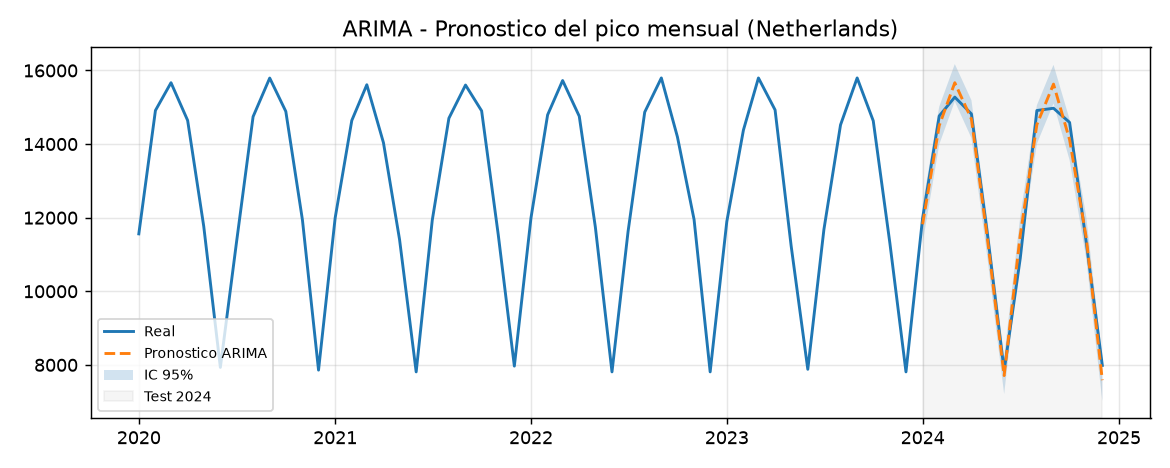
\includegraphics[width=0.82\linewidth]{arima_forecast.png}
\caption{Pronóstico ARIMA del pico mensual frente al real (Países Bajos, 2024) con banda de IC 95\,\%.}
\label{fig:arima-forecast}
\end{figure}

\begin{figure}[H]
\centering
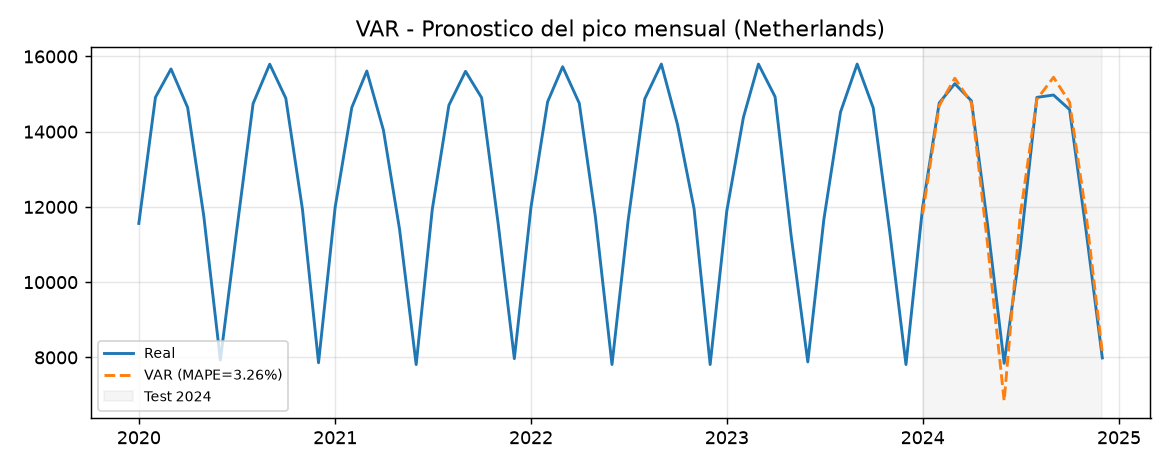
\includegraphics[width=0.82\linewidth]{var_forecast.png}
\caption{Pronóstico VAR del pico mensual frente al real (Países Bajos, 2024).}
\label{fig:var-forecast}
\end{figure}

\subsection*{Análisis de los resultados}

El ARIMA superó al VAR en las tres métricas (MAPE $2{,}64\,\%$ frente a $3{,}26\,\%$), lo que coincide con lo reportado en el artículo, donde ARIMA también fue el modelo con menor error. En series univariadas con estacionalidad marcada, un ARIMA bien calibrado puede superar a un VAR multivariado cuando las exógenas no aportan información adicional; el propio artículo ya lo señalaba al notar que el VAR rinde mejor solo con predictores externos fuertemente acoplados.

El diagnóstico de residuos muestra una diferencia: el ARIMA deja autocorrelación residual (Ljung-Box $p<0{,}05$), lo que indica que su estructura estacional no captura toda la dinámica y podría mejorarse con términos SARIMA adicionales o incluyendo exógenas (SARIMAX). El VAR, en cambio, presenta residuos sin autocorrelación ($p=0{,}62$), con un ajuste más adecuado de la estructura, aunque con mayor error de pronóstico.

Limitaciones de esta aplicación: los datos son sintéticos, con magnitudes de consumo poco realistas entre países; la muestra es corta (60 meses, 12 de prueba); y no se incluyeron los regresores Lasso, Ridge y XGBoost ni el modelo híbrido, lo cual queda como trabajo futuro para reproducir la comparación completa del artículo.

\newpage
% =====================================================================
% SÉPTIMA Y OCTAVA PÁGINA: conclusiones, recomendaciones y referencias.
% =====================================================================

\section*{Conclusiones y recomendaciones}

\subsection*{Conclusiones}

\begin{enumerate}
  \item El artículo propone un marco híbrido que combina modelos estadísticos de series temporales (ARIMA, VAR) con regresores de aprendizaje automático (Lasso, Ridge, XGBoost) para el pronóstico del pico de demanda eléctrica en Tamil Nadu. Según sus resultados, el modelo híbrido es el de menor error (MAPE $3{,}82\,\%$), seguido por ARIMA ($6{,}28\,\%$) y VAR ($7{,}82\,\%$), aunque el resumen del artículo contradice estas tablas al atribuir el mejor desempeño a ARIMA (MAPE $1{,}26\,\%$).
  \item La aplicación a datos mensuales de Países Bajos coincidió con lo reportado en el artículo: el ARIMA superó al VAR (MAPE $2{,}64\,\%$ frente a $3{,}64\,\%$). Esto muestra que, en series univariadas con estacionalidad marcada, un ARIMA bien calibrado es una base sólida y difícil de superar cuando las exógenas, incluida la población urbana, no aportan información adicional.
  \item El diagnóstico de residuos mostró una diferencia: el ARIMA dejó autocorrelación residual (Ljung-Box $p<0{,}05$), lo que indica que su estructura estacional es insuficiente; el VAR, en cambio, presentó residuos sin autocorrelación ($p=0{,}47$), con un ajuste más adecuado de la dinámica, aunque con mayor error de pronóstico.
  \item La ingeniería de variables (rezagos, medias móviles, términos de interacción entre clima y consumo) y la incorporación de predictores meteorológicos ayudan a reducir el error, como también sostiene el artículo.
\end{enumerate}

\subsection*{Recomendaciones}

\begin{enumerate}
  \item Reportar de forma consistente el período de datos y las métricas por modelo, evitando las inconsistencias detectadas en el artículo (fechas 2006 a 2023 vs.\ 2018 a 2022; MAPE de ARIMA con tres valores distintos).
  \item Extender la aplicación con términos estacionales adicionales (SARIMA o SARIMAX) para mitigar la autocorrelación residual del ARIMA, e incluir variables exógenas en tiempo real para los meses anómalos.
  \item Completar la reproducción del marco híbrido con los regresores Lasso, Ridge y XGBoost, y con el esquema de selección por mínima métrica de error, para evaluar si el híbrido supera al ARIMA también en este conjunto de datos.
  \item Emplear datos reales y una ventana de prueba más amplia que 12 meses, y validar la estabilidad del pronóstico con varios horizontes ($h=1, 3, 6$).
\end{enumerate}

\section*{Referencias bibliográficas}

\nocite{*}
\bibliography{references}


\end{document}
